\section{Localised Processing, Storage and Classification}
In this section the report will discuss the implementation of the Edge Node and all facilities within it.
\subsection{Setting up the Environment}
In order to simulate an Edge Device rather than a separate piece of hardware, a Virtual Machine (\textbf{VM}) can be setup on the laptop. However, the virtual machine is just to represent an Edge Device running an embedded UNIX OS. In this scenario using Vagrant in conjunction with VirtualBox allows us to setup and use a virtual Ubuntu system. This is all to emulate an edge device such as a Raspberry Pi or a server running at the remote location. The guide on the Vagrant website takes the developer step by step through the setup stages of getting the VM setup. \cite{installing_vagrant}. 

Once this is setup, the Greengrass Core (GGC) can now be setup and ran on the \textit{Edge Device}. First the Greengrass group was setup via the IoT Core page on AWS and then a group was setup using the default settings. When the group is first initialised, a zip file filled with correct certifications and configuration files is produced. These files must be placed into the installed GGC folder on the Edge Device under \textit{/greengrass/certs} and \textit{/greengrass/config}. Then the Greengrass Core can be started up by running the program stored at \textit{/greengrass/ggc/core/greengrassd}.

\begin{figure}[ht]
    \centering
    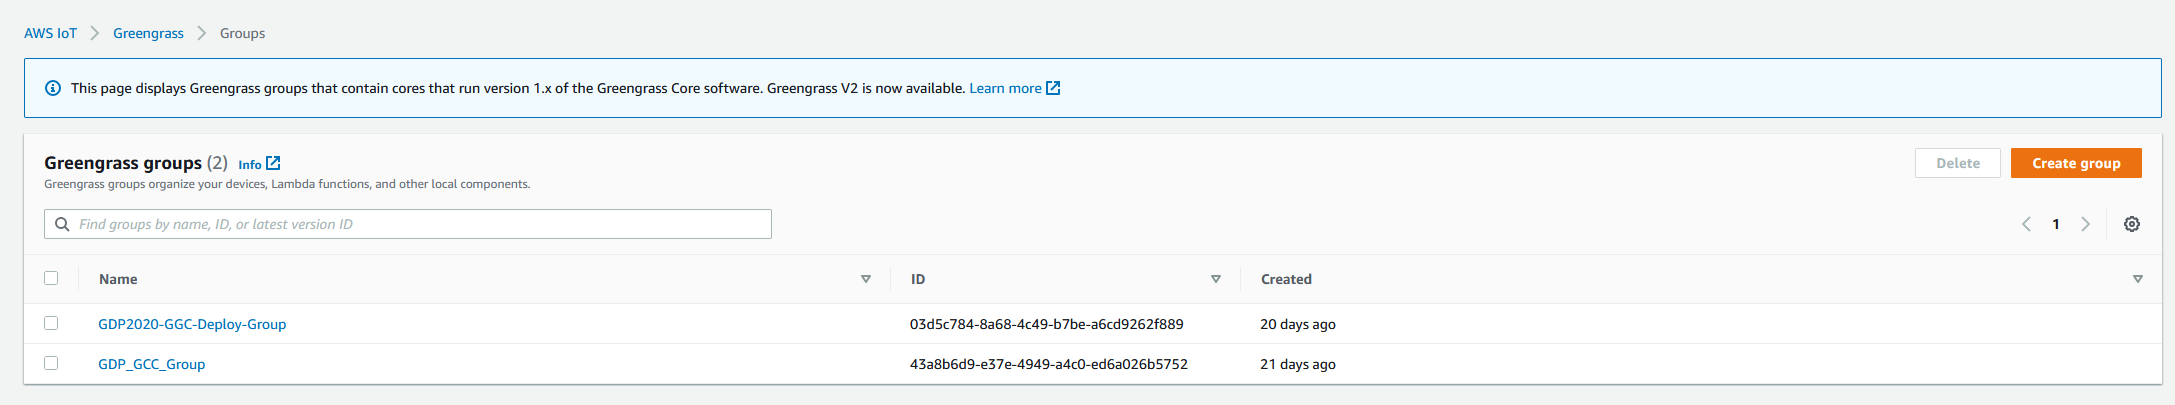
\includegraphics[width=1\linewidth]{pages/Chapter4/Chapter 4 Images/greengrass_group.png}
    \caption{Setting up Greengrass Group on the AWS IoT Core dashboard}
    \label{fig:my_label}
\end{figure}

There are some additional steps that need to be run in terms of installing the pre-requistes and give the Greengrass Group User access to run programs. These instructions and the specific commands can be found in the AWS Documentation in Greengrass Deployment \cite{greengrass_deployment}.

\subsection{Attaching Lambda Functions to the Greengrass Group}
Once the Greengrass Group is setup, a Lambda function to run on the device can be setup as long as the runtime requirements are also on the device (e.g. nodejs12.x must be installed to run NodeJS at the Edge Device). Then on the Greengrass Group dashboard a new existing Lambda function is attached. as seen in Figure \ref{fig:adding_new_lambda_to_ggc}. Step 1 is to add the Lambda function, then attach an existing Lambda function from the provided list. This Lambda function must already have been created in the AWS Lambda Dashboard.

\begin{figure}[ht]
    \centering
    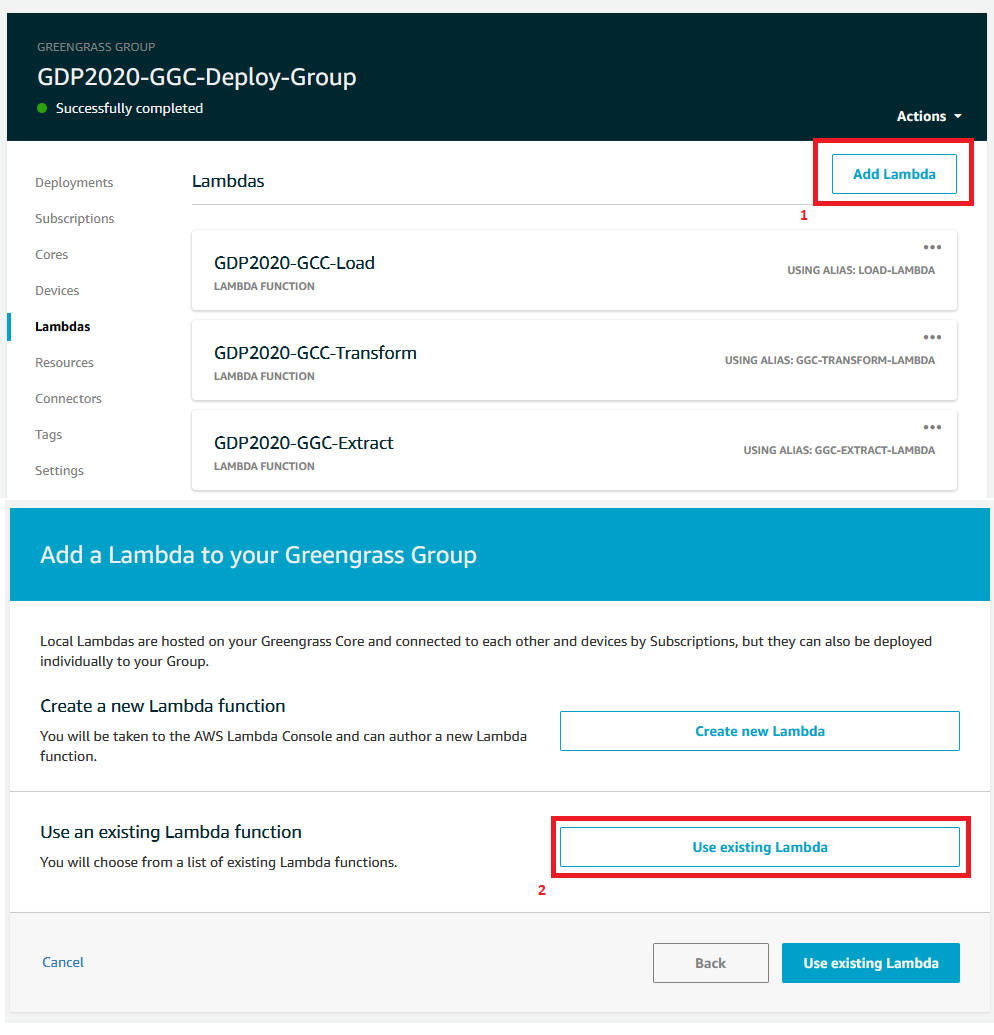
\includegraphics[width=100mm, scale=0.5]{pages/Chapter4/Chapter 4 Images/greengrass_new_lambda.png}
    \caption{Adding a new Lambda Function via the Dashboard.}
    \label{fig:adding_new_lambda_to_ggc}
\end{figure}

Once this is complete, using the drop down in the top right of the Greengrass Groups dashboard allows you to deploy or re-deploy an existing version. Shown in Figure \ref{fig:deploy_on_dashboard}.

\begin{figure}[ht]
    \centering
    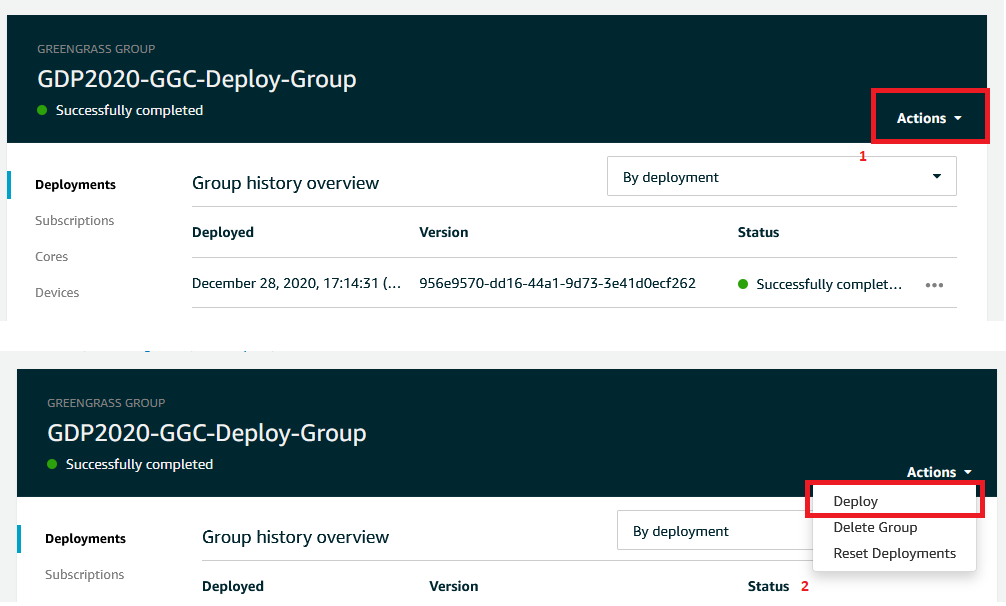
\includegraphics[width=100mm, scale=0.5]{pages/Chapter4/Chapter 4 Images/deploy_group.png}
    \caption{How to deploy the Greengrass Group via the Dashboard}
    \label{fig:deploy_on_dashboard}
\end{figure}


To enable the GGC to access the hosts' local resources, \textit{Local Resource Access} must be setup on the group. Local Resource Access is a way for the containerised Greengrass Core to gain access securely to a specific directory outside of the container. This is done by setting up a \textit{src} directory on the host, and a matching \textit{dest} directory on the Greengrass device. This process can be seen in Appendix F [\ref{appendix:ggc_lra}]. A folder within the containerised GGC is labelled as \textit{'dest/LRAtest/...'} and outside of the container on the host device (or VM in our case) is a similar folder \textit{'src/LRAtest/...'}. These two directories are linked with each other. Files stored into the former location will be also seen on the host machine under the latter location and visa versa.

The next following sections will discuss how to setup each Lambda function.
\begin{itemize}
    \item Extract - \ref{extract_fn_impl}
    \item Transform - \ref{transform_fn_impl}
    \item Load
    \item Local ML Inference
    \item Remote ML Inference
    \item NodeJS Web Server Application
\end{itemize}


\subsection{Extract Function}
\label{extract_fn_impl}
The first localised Lambda function is mainly to remove the .db file to JSON files conversion processing requirement from the user device (that is if the device was capable in the first place), and places the load onto the Edge Node. As this is the first implemented Lambda Function, one requirement to run any Lambda is the requirement to include the Greengrass SDK. This is done by uploading a zip file to the Lambda function which includes the main program file and the SDK Folder as seen in \ref{fig:ggc_sdk_inclusion}
\begin{figure}[ht]
    \centering
    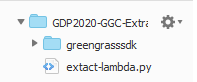
\includegraphics{pages/Chapter4/Chapter 4 Images/LambdaFns/ggc_sdk_inclusion.png}
    \caption{How the zipped  directory needs to be uploaded.}
    \label{fig:ggc_sdk_inclusion}
\end{figure}

This setup must be completed for each function, and any external python dependencies must also be included in this zip file. Once the setup is complete, then the python application can be developed. The extract-function python implmentation follows the dataflow shown in \ref{fig:lambda_extract_fn}.

\begin{figure}[ht]
    \centering
    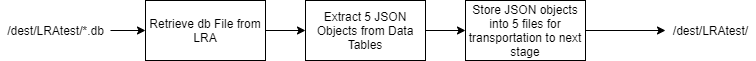
\includegraphics[width=1\linewidth]{pages/Chapter4/Chapter 4 Images/LambdaFns/extract-fn.png}
    \caption{Extract Lambda Function Block Diagram}
    \label{fig:lambda_extract_fn}
\end{figure}

The implementation for this function is very similar to the implementation for the Laptop-To-Cloud Pipeline with the main changes being the setup required for the local resource access from the edge node.

\subsection{Transform Function}
\label{transform_fn_impl}
The transform function implementation follows the block diagram shown in \ref{fig:lambda_transform_fn} with the main points of implementation being where the output file, the compressed JSON object with all the separate data tables' data in one, is placed. The output file is placed into 3 locations for usage by other Lambdas. It should be noted that it was chosen to replicate the 3 output files so as to avoid any issues with access from multiple locations (separate Lambda functions). However, this leads to a longer run-time as the write operation has to be run three times rather than 1, but is only a problem for very large files as is seen later in the testing stages.

\begin{figure}[ht]
    \centering
    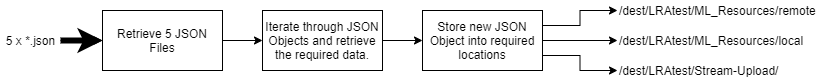
\includegraphics[width=1\linewidth]{pages/Chapter4/Chapter 4 Images/LambdaFns/transform-fn.png}
    \caption{Block Diagram of Transform Function at the Edge Node}
    \label{fig:lambda_transform_fn}
\end{figure}


\subsection{Load Function}
\label{load_fn_impl}
For this Lambda function, the python library requests is used and so the dependency folder must be extracted from several ways. 
\begin{itemize}
    \item Copy directly from developer's Python dependencies list.
    \item Setup a virtual environment for Python and install all dependencies will then be stored locally in that virtual environment. These can then be zipped up and extracted and the developer's program injected into the zipped folder for upload to the Lambda function.
\end{itemize}

Since the requests library is a small library with no build-for-os/host-architecture requirement (this will become an issue later for the XGBoost library), the first implementation method was followed and copied directly from the python-libraries list after doing using \textit{pip install requests} and \textit{pip show requests} to ensure no other sub-dependencies were required. The final zipped folder to upload to the Load-Lambda function is shown in Figure \ref{fig:lambda_requests_ggc_sdk}.

\begin{figure}[ht]
    \centering
    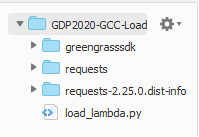
\includegraphics{pages/Chapter4/Chapter 4 Images/LambdaFns/ggc_sdk_requests_inclusion.png}
    \caption{File structure for Upload to Load Lambda with Requests and GGC SDK}
    \label{fig:lambda_requests_ggc_sdk}
\end{figure}

The implementation of the load lambda function follows the block diagram in Figure \ref{fig:lambda_load_fn}. Environment variables can also be setup within the AWS Lambda dashboard to ensure no details of the private key are released without intention. 

\begin{figure}[ht]
    \centering
    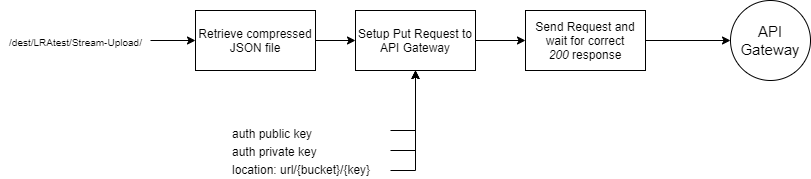
\includegraphics[width=1\linewidth]{pages/Chapter4/Chapter 4 Images/LambdaFns/load-fn.png}
    \caption{Block Diagram of Load Function at the Edge Node}
    \label{fig:lambda_load_fn}
\end{figure}


\subsection{Local-ML Function}
%looooooooooooong%
For the Local-ML Lambda function there are several steps that need to be completed. \begin{enumerate}
    \item Import the Sagemaker Model from either Sagemaker or S3
    \item Setup Python Dependencies for use of XGBoost Python Library at the Edge, these must be built specifically for the end-device architecture and OS. (e.g. Linux on x84\_64 architecture)
    \item Upload Zipped File of Dependencies and python program file
    \item Complete Program and Deploy to Greengrass Core.
\end{enumerate}
These 4 stages of the process describe the implementation process, with the second stage being the most difficult and will take the longest. Since the XGBoost and its sub-dependencies must be built from scratch due to usage of C program files must be built for the target device. 



The first stage is as follows. In the development stages of Sagemaker Model Training and Deployment, a model is produced as a zip file. This zip file containing the ML-Model can be imported direclty into the Greengrass Group as a resource to be used within the container environment. It can be either imported from S3 or directly from Sagemaker. This is seen in Figure \ref{fig:ggc_model_import} where the ML model must also be attached to a Lambda function for it to be accessible by that Edge-based Lambda function. First the \textit{'Add machine learning resource'} must be clicked, then the model name entered and a choice must then be made of the source location of the model. In the figure, the model is uploaded from a provided S3 bucket and location within it. Then the local path within the Greengrass container is also chosen. This is for usage within the attached Lamda function to the Machine Learning Resource, to open the directory with the model.

\begin{figure}[ht]
    \centering
    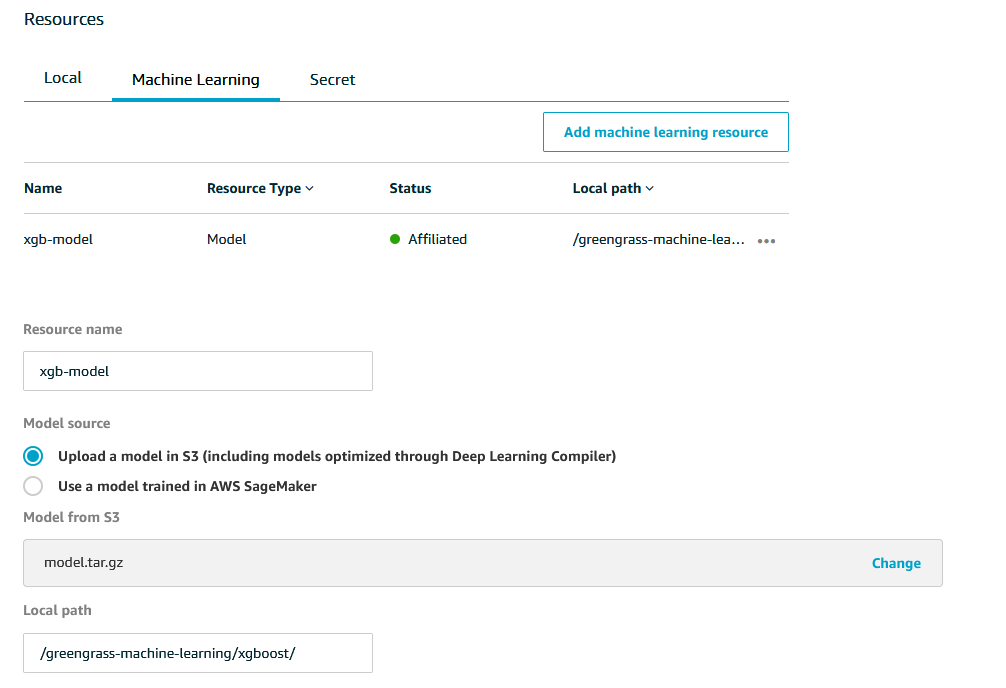
\includegraphics[width=1\linewidth]{pages/Chapter4/Chapter 4 Images/LambdaFns/xgboost_model_import_ggc.png}
    \caption{Importing XGBoost Model from S3 into the Greengrass Group as a local Resource}
    \label{fig:ggc_model_import}
\end{figure}

Once the ML-Model is attached and a Lambda function to handle the Local-ML Inference is also attached, then the dependencies can be built. First an EC2 instance is instantiated in order to help the developer build and pack the dependencies. The developer must set up a virtual python environment so that the python dependencies are installed remotely and any sub-dependencies are also present (as these must also be zipped as previously mentioned). The developer must then also install Python 3.7 rather than Python 3.8 within the Virtual environment as Greengrass at the time of writing this report only supports Lambda functions with a runtime of Python3.7. Once the virtual environment is setup and any sub-depencies or other required libraries are setup. In this case, the dependencies required are:
\begin{itemize}
    % \item \textit{xgboost}
    \item \textit{numpy}
    \item \textit{scipy}
    \item \textit{six}
    \item \textit{pkg\_resources}
\end{itemize}
Once these dependencies are setup, then one must download the XGBoost source files from the github and use cmake to manually compile the program for the Amazon Linux OS running on x86\_64 architecture. It should be noted that cmake will also need to be downloaded and compiled from scratch. The exact commands to achieve this can be found on a post by Lucas Silva \cite{silva_2019}. However, these commands must be adjusted for our specific sub-dependencies, and the article uses Python 3.8 rather than 3.7, to install Python 3.7 it requires further adjustment of the commands as seen in the article by Rahul Kumar of installing Python 3.7 on Amazon Linux. \cite{kumar_2020} 

Following the instructions provided produces a zip file that can be uploaded to an S3 bucket for retrieval from the EC2 instance and then uploaded into Lambda. Once this is complete the implementation of the program can begin. The implementation of the main program follows the block diagram shown in Figure \ref{fig:localml-function}. The block diagram shows how the program running in the Lambda function will operate. First it must retrieve the model and the JSON file from the appropriate local directories in the Greengrass container. Then apply some pre-processing to make them fit for usage. The XGBoost python package then comes with a predict function that allows us to input the data parameters for one timestamp and per MAC Address. This output result can then be stored locally or passed to the OTT Application or to the Web server application for live-viewing of the results as well as comparisons to the Remote-ML timings.

\begin{figure}[ht]
    \centering
    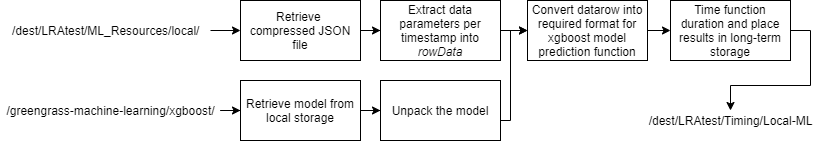
\includegraphics[width=1\linewidth]{pages/Chapter4/Chapter 4 Images/LambdaFns/localml-fn.png}
    \caption{Block Diagram for Local-ML Function at the Edge Node}
    \label{fig:localml-function}
\end{figure}
%Import of Sagemaker model into greengrass via dashboard
%How it can be accessed
%Setup of Dependencies using Cloud-Based resources, ensure version for python3.7, ensuring also size of lambda zip is less than 250mb as a hard limit from them
% any more than 50mb must be uploaded from s3

\subsection{Remote-ML Function}
After the setup to include the requests library is completed. As well as the API Gateway setup to redirect data from the Edge Node to a Cloud-based Lambda that will redirect the data securely to the Sagemaker Endpoint, a similar implementation to that \ref{fig:lambda_load_fn} is used, however the location address is changed. The response from the endpoint is also how the Lambda function will receive the results of the Machine Learning Model's output. A code snippet shows how the request can be setup by reading the JSON file and then sending the data as requested to the API Gateway to be processed by the Cloud-Based Lambda as shown in Listing \ref{lst:edge_remote_ml}
\begin{lstlisting}[language=Python, caption={Sending Data to API Gateway to Invoke Cloud-Based Lambda for Sagemaker Endpoint}, label={lst:edge_remote_ml}]
with open(jsonLoc, 'r') as jF:
                payload = json.dumps(json.loads(jF.read()), separators=(',',':'))
            client.publish(
                topic='mlEndpoint/checkFile', 
                queueFullPolicy='AllOrException', 
                payload="Opened file success!")
            headers = {
                'Content-Type': "application/json, text/plain",
                'Host':"vnl7ji5sz2.execute-api.eu-west-2.amazonaws.com",
                }
            start = time.time()
            response = requests.request(
                                    "POST", url, 
                                    data=payload, 
                                    headers=headers
                                    )

\end{lstlisting}
The implementation for the Cloud-Based Lambda which is responsible for further pre-processing to fit the model is shown in the later section for implementation of Cloud-Based services. The Cloud-Based Lambda interacting with the Sagemaker endpoint will then return the result of the classification in the form of a value of 0 to 4 inclusive corresponding to a classification of the data throughput as discussed in the Machine-Learning system design section.


\subsection{MQQT to Web Application}
The primary method for communication from the edge node to the cloud, and from service to service at the Edge Node is via transportation of MQQT packets. For the most part, the messaging system has been abstracted away from us and so only a subscription topic is used and the data object to be transported. Each service can subscribe to a topic which allows it to listen and be triggered by the new packet or allows the service to successfully publish to the topic.

This means it can be used for debugging as well as real-time application usage. These messages are a clean way to send small data items that cannot be intercepted from outside of the containerised Greengrass Core, hence the usage within this system. The first set of subscriptions set and to be used is the debugging layer and error checking. During implementation of each Lambda function above, subscriptions and messages were sent to monitor progress of the Lambda function in any of the retrieving, processing or storing stages inside each Lambda function. The debugging subscriptions can be seen in Figure \ref{fig:cloud_mqqt_layer}. In this diagram, each Lambda function that is attached to the Greengrass Group as well as the topic it is subscribed onto.

\begin{figure}[ht]
    \centering
    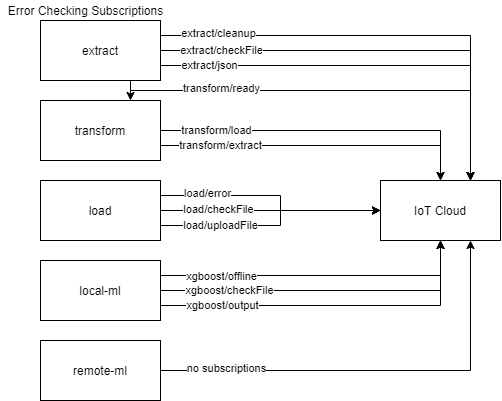
\includegraphics[width=1\linewidth]{pages/Chapter4/Chapter 4 Images/LambdaFns/iot_cloud_mqqt.png}
    \caption{Subscriptions from Lambda to IoT Cloud Service for Debugging and Error Checking}
    \label{fig:cloud_mqqt_layer}
\end{figure}

\subsection{Web Server Application for Live Data Viewing}


\section{Edge Node Technology Exploration - AdvantEDGE} %Syuhada's Section
\subsection{AdvantEDGE Implementation}
The mobile edge emulation platform required a system that runs on bare Linux operating system (OS) or within virtual machines (VMs) and may be installed on a single Kubernetes (K8s) node or a cluster of K8s nodes. The system requirements to install AdvantEDGE include building the runtime environments – Ubuntu, Dockers, Kubernetes, Helm and NVIDIA GPU support. With the system set up, one can clone AdvantEDGE repositories into local host before installing and configure the meepctl tool, a command-line interface (CLI) applications to control the platform. 
Configuring meepctl to the node’s IP address and the directory on the local host, AdvantEDGE binaries can be built to generate the micro-services, as well as the front-end web application. AdvantEDGE micro-services fall into two categories: core and dependencies. Prior to deploying AdvantEDGE core components, dependencies to creates micro-services required to run AdvantEDGE can be deployed onto K8s cluster with meepctl tool and then dockerize these micro-services into container images to be stored into a configured Docker registry. The platform GUI then can be accessed through the standard browser.

To emulate the physical system model, a scenario of the network model can be built by configuring each of the elements needed such as the Internet Cloud, operator, zones, PoA and the edge nodes,  connecting the simulation platform to the physical running native edge application on the server. 

This edge native application is the same python script used in the AWS IoT Greengrass edge node that able to extract, transform and load (ETL) the data before sending them off to the distant cloud. However, prior to connect the edge application to the AdvantEDGE, the python application required to be containerized into Docker image, stored in the Docker registry. Dockerfile, a text document without the extension that contains all the commands a user could call on the command line to assemble an image, has to be created, placed together in the same directory as the python script and requirement.txt. Requirement.txt is a file that contained the dependencies that the python script needs to run successfully. This file can be first generated on the command line by “pip freeze >> requirement.txt”. 

\begin{figure}[ht]
    \centering
    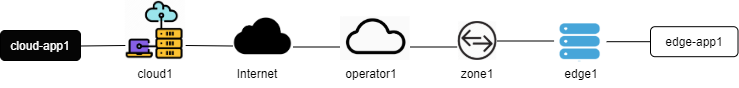
\includegraphics[width=1\linewidth]{pages/Chapter4/Chapter 4 Images/Scenario.png}
    \caption{Scenario created in AdvantEDGE to emulate the physical network topology.}
    \label{fig:AdvantEDGE_scenario}
\end{figure}

On AdvantEDGE web GUI, a scenario is created as Figure \ref{fig:AdvantEDGE_scenario}.
The cloud and edge application are connected to the real applications through the configuration where detailed specifications such as group container name, port, protocol, command and arguments need to be provided before deploying the scenario into the sandbox. The scenario then can be deployed once the button on the right top turns green, indicating the server is all good. When executed, one can set the source node and the destination node, to measure the latency, data throughput and traffic metrics in between the nodes after configuring the elements’ network characteristics which can indirectly configure the router. It displays instantaneous measurements for round-trip ping time on the graph if we select to display on the Network Metrics Point-to-Point.

\begin{figure}[ht]
    \caption{Example of Dockerfile}
    \centering
    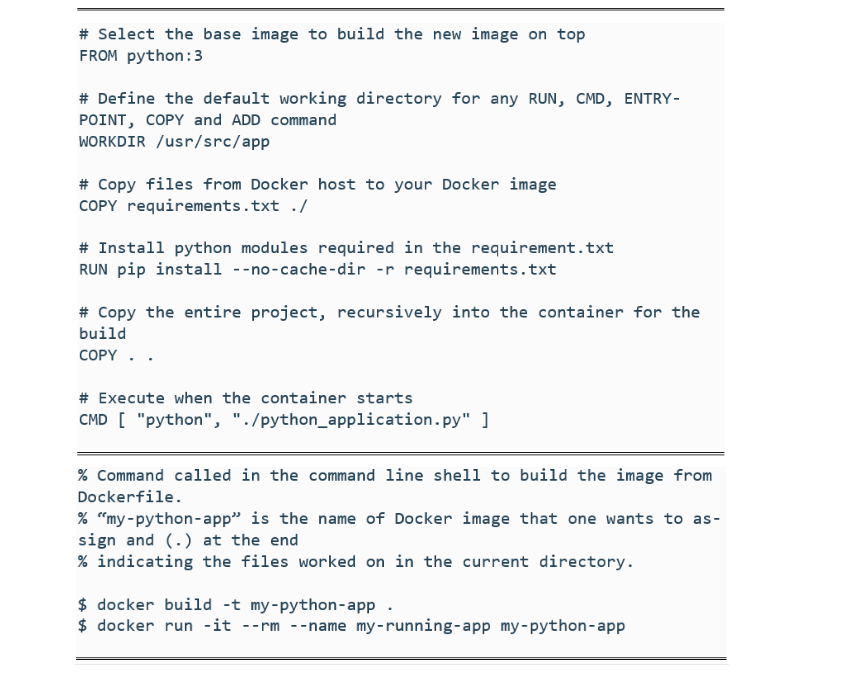
\includegraphics[width=1\linewidth]{pages/Chapter4/Chapter 4 Images/Dockerfile.PNG}
\end{figure}

Once this is setup, the Greengrass core can now be setup and ran on the \textit{Edge Device}. First the Greengrass group was setup via the IoT Core page on AWS and then a group was setup. When the group setup 

